%silber messreihe 2: konstante n(0)exp(...) lässt auf zu kurze Wartezeit schließen (bei messreihe 1 waren das noch so 39)\section{Durchführung}
\begin{figure}
    \centering
    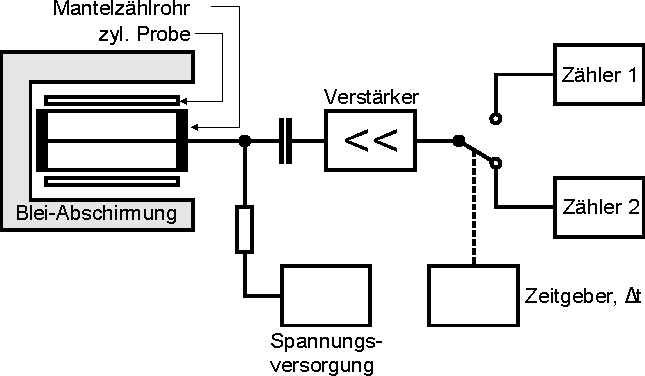
\includegraphics{Abbildungen/Schaltplan.pdf}
    \caption{Aufbau der Messanlage \cite{man:v702}}
    \label{fig:Aufbau}
\end{figure}
Die Messungen erfolgen mit der In Abb. \ref{fig:Aufbau} skizzierten Apparatur